%%
\documentclass{aiaa-tc}% insert '[draft]' option to show overfull boxes
% \documentclass{article}% insert '[draft]' option to show overfull boxes
%%

% list packages between braces
\usepackage{graphicx}
\usepackage{varioref}%  smart page, figure, table, and equation referencing
\usepackage{wrapfig}%   wrap figures/tables in text (i.e., Di Vinci style)
\usepackage{threeparttable}% tables with footnotes
\usepackage{dcolumn}%   decimal-aligned tabular math columns
\newcolumntype{d}{D{.}{.}{-1}}
\usepackage{nomencl}%   nomenclature generation via makeindex
\makeglossary
\usepackage{subfigure}% subcaptions for subfigures
\usepackage{subfigmat}% matrices of similar subfigures, aka small mulitples
\usepackage{fancyvrb}%  extended verbatim environments
\fvset{fontsize=\footnotesize,xleftmargin=2em}
\usepackage{lettrine}%  dropped capital letter at beginning of paragraph
%\usepackage[dvips]{dropping}% alternative dropped capital package
%\usepackage[colorlinks]{hyperref}%  hyperlinks [must be loaded after dropping]
\usepackage{amsmath}

%% Daoru added the following package
\usepackage{multirow}
%%

\begin{document}

\title{CSCI545 Robotics Final Project Report\\
	Robotic Motion Planning}

 \author
{		May Ang%
		\hspace{3pt},
		Thomas Collins%
		\hspace{3pt},
		Justin Garten%
		\hspace{3pt},
		and Michael Joyce%
		\\
		\normalsize\itshape
		University of Southern California, Los Angeles, CA, 90007, USA\\
}
\maketitle

\begin{abstract}
In a world gone mad, one project dared to impose its own brand of
brutal justice on a world many thought too far gone to save.
\end{abstract}

\section{Introduction}
\label{Introduction}

\subsection{Background}

Robots are no longer confined behind striped yellow lines
with flashing lights to keep soft humans away from the moving
parts. They operate in busy hospital hallways, kitchens, and homes
with pets, children, and clutter in a constant state of motion. As
such, the ability to evaluate and interact with those dynamic environments is
increasingly essential for successful operation.

There are a number of possible approaches to this, many of which are
strongly influenced by the risks of the environment, nature of the
task, and the type of information to which the robot has
access. If uncertain, should it simply stop and wait for instructions?
Should it push through, trusting others to get out of its way? An
industrial bot capable of ripping through a wall might have very
different issues than a robotic vacuum which will at most scuff a
floorboard.

\subsection{Problem Description}

Issues relating to navigation and motion planning run up and down the entire
robotic stack. We chose to focus on the high-level planning aspects of the problem, particularly those relating to dynamic, noisy environments. Our primary approach was to explore, extend, and
evaluate three broad categories of methods for navigating in a dynamic
environment: potential fields, Markov decision processes, and
reinforcement learning.

\subsection{Robocode Environment}

As the environment for our experiments, we chose to work with a small
framework called Robocode \\(http://robocode.sourceforge.net/). This system is designed for small-scale
simulated robotic tank battles. Users of the system are able to write
the central processing loops for the robots which have access to
standard sensors, weapons, and motion controls. 

Several features in particular appealed to us. It's semi-continuous underlying state
representation (locations as doubles) gave us flexibility in
terms of laying a grid over the environment rather than existing in a
pre-defined grid. Critically, this made it far easier to experiment
across methods which required discretization (MDPs and Q-learning) and
those which did not (potential fields).

The motion controls proved to be similarly flexible, lending
themselves to discretization when necessary, while leaving access to
the low-level controls where appropriate.

The sensors offered a range of options, providing a flexible base
model which was easily extended to account for the particular
structure of individual
experiments. This was abstracted in the Robocode context with the
concept of radar. Basically, each bot had a narrow-band sensor which could be rotated 360 degrees to provide a sweep of the environment and in internal sensor to keep track of its (x, y) position on the battlefield at all times.

Finally, the visualization was an appealing fringe benefit, providing
rapid feedback on experiments and allowing us to more easily evaluate
and iterate.

One of the first steps in this project was to evaluate the possible
environments to work in. As our aim was to focus in on the planning and navigation algorithms,
we wanted to work in a context which allowed us to abstract and
encapsulate as many
surrounding issues as possible. After a certain amount of exploration, we did
in-depth evaluations of three options: ROS, a simple grid world, and
Robocode.

For ROS, the primary issue was the potential length of time setup
would require. As none of us had extensive prior experience, our
initial efforts suggested that we might end up spending a good portion
of project time on learning the tools. While this is an environment that all
of us were interested in, even in the best case it would not have left
us a great deal of time to explore the planning and navigation
algorithms we were primarily interested in.

For a custom grid world, the issue was the risk of getting bogged down
in implementation details and the inability to take advantage of any
existing features, particularly in terms of visualization.

We settled on the Robocode environment as a good compromise for our
needs. It proved to be a solid choice as it provided us with the
ability to add in features as required while working in a simple
space when needed, not much more complicated than a basic grid world.


\subsection{Report Outline}
In the following three sections, we discuss our efforts to explore
this task using Potential Fields, Markov Decision Processes (MDPs) and
reinforcement learning, specifically Q-learning.

\section{Potential Fields}
\label{Potential Fields}

\subsection{Setup}
The implementation of Potential Fields in Robocode went through a number of steps before coming to a satisfying conclusion. The implementation relies on a few assumptions that Robocode makes possible. First, Robocode always allows the robot get its exact $x$ and $y$ coordinates via \verb|getX()| and \verb|getY()| respectively. The heading of the robot can be gathered from a call to \verb|getHeading()|. The potential field implementations focus on manipulating the heading of the robot and the speed settings to get effective navigation and obstacle avoidance. Potential fields didn't require any special setup like the other methods tested, so jumping into the development was mostly painless.

% Experiments
\subsection{Experiments}
The first goal of potential field implementation was getting a simple proof of concept working in Robocode. The environment was unfamiliar, but fairly simple, so this didn't pose too great a problem. The initial tests were simple single agent environments with a stationary goal. To encode the notion of a ``goal'' in Robocode a stationary bot was used. To calculate the angle of rotation needed to point towards the goal, the robot coordinates and goal coordinates were subtracted and passed to the arctangent variant \verb|Math.atan2()|. This could be used to modify the current heading value, and thus turn the robot towards the goal. 

While the initial tests worked, the performance was less than stunning. The simple motion model in Robocode was used as opposed to the advance, which meant that all the robot actions blocked. For this simple example it didn't pose much of a problem, but it made scaling the speed as the bot approached the goal less than ideal. It did cause problems in later tests and would eventually be changed.

The next reasonable step seemed to use a moving goal since a stationary goal wasn't especially interesting to watch. Again, as with all the tests, a simple robot was used to implement the goal. It was coded to follow a simple pattern around the environment as quickly as possible. The test robot would rotate in a circle until it located the goal. Once the goal was found, it would do its best to continue heading towards the goal. 

It was this test that made it evident that the simple motion model wasn't sufficient. While tasks like sweeping the radar can be performed in the simple model, they eat up ticks that the robot could spend doing something else. The bot would end up rotating the radar for one tick, then turning with another tick, and then moving forward with yet another tick. 

\begin{figure}[htb]
\centering
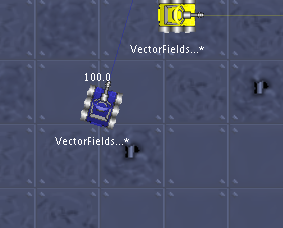
\includegraphics[width=0.5\textwidth]{images/SimpleRadarFailure}
\caption{Notice that the blue robot has lost track of the goal and is tracking an older position.}
\end{figure}

In an effort to save ticks and make the motion of the robot smoother, the radar was locked facing forward so the bot would always scan the direction it faced. However, the bot would sometimes lose track of the goal if it passed to close or made sudden direction changes. In addition, because the actions in the simple motion model block, the speed had to be set to the lowest possible setting. If it wasn't, the robot would attempt to move forward some number of units in the environment before doing another radar sweep. This resulted in the robot losing track of the goal quite quickly. So the decision ended up being between extremely slow motion that eventually lost track of the goal, or slightly faster motion that quickly lost track of the goal. Either way, these results weren't satisfying and it was evident that a new approach was needed.

After doing some research, it was decided that the advanced motion model was needed to improve the implementation. Unfortunately the examples and tutorials provided for Robocode only touch on the simple motion model. With a bit of persistence the model was understood enough for implementation. Instead of actions blocking, the robot queues up actions until a call to \verb|execute()| or \verb|scan()| is encountered. Then it attempts to execute all the queued commands simultaneously while obeying the physics of the environment. 

The initial test of the advanced motion model used a moving goal. In order to minimize the amount of time the robot spent following the old position of the goal, the radar was constantly rotated at maximum speed independent of the position and heading of the bot. This allowed for much improved performance. The robot's speed could be increased quite a significant amount without worry that it would overshoot and hit the goal or lose track of its location. That being said, the motion of the tracking robot was not perfect. There was often a delay in recognizing the changing position of the goal. 

The main issue was the wasted ticks sweeping the radar through empty space. This would cause the robot to track old positions while the radar completed its sweep. What was needed was a perfect radar lock so that the robot would always have the exact position of the goal. While the performance with the sweeping radar was satisfactory, it was felt that perfecting the situation where there weren't obstacles would only make future implementations easier and cleaner.

\begin{figure}[htb]
\centering
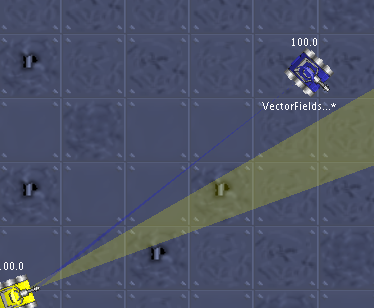
\includegraphics[width=0.5\textwidth]{images/RadarLock}
\caption{The blue tracking robot has located the goal with its radar, even though it is facing a different direction. It will never lose track of the goal now that it has a lock.}
\label{Radar Lock Example}
\end{figure}

To implement a radar lock that would never slip required simple algebraic manipulation of the state information present when a onScannedRobot event occurred. Whenever the goal was scanned, the radar's rotation was set to the tracking robot's heading added to the scanned ``goal'' robot's heading minus the radars heading. More succinctly, $NewRadarHeading = RobotHeading + GoalHeading - CurRadarHeading$. This angle was then normalized so that it fell within the range of $[-\pi, \pi]$. This caused the radar to constantly rotate towards the direction that the goal was navigating so the radar never slipped and the goal was never lost. It also minimized the amount that the radar needed to be rotated so that less ticks were spent uselessly spinning the radar.

Performance with the radar lock implemented was near as perfect as the simulation would allow. The robot could travel just as fast as the goal and never lose track of the location. In fact, the max speed of the tracking robot had to be turned down to ensure that it didn't catch up to and crash into the goal. In addition, because the tracking was so smooth, the speed of the bot could be appropriately scaled based on distance to the goal without fear of any blocking actions causing a loss of the goal or a slow scan resulting in a crash.

Once the moving goal tracking had been sufficiently implemented, the next obvious step was obstacle avoidance. As with the goal, obstacles were nothing more than stationary or moving robot entities added to the simulation. The initial implementation of obstacle avoidance was simplified to include a single stationary obstacle and a stationary goal. This ensured that all issues with obstacle avoidance could be ironed out before dealing with the issues of adding a moving goal to the equation. 

When a robot was scanned by the tracking robot that wasn't recognized as the goal, the robot would calculate and save the coordinates of that bot and assume it was an obstacle. Goal or obstacle recognition was handled in the onScannedRobot event handler by accessing the scanned object's name. The appropriate name values were simply coded into constants and checked whenever something was scanned.

Since the location of the obstacle was stored as a pair of coordinates, the distance from the robot to the obstacle could be calculated during each iteration of the navigation loop. This distance value was checked against a previously defined threshold value that determined if the navigating robot was within the area of affect of the obstacle. The formula used to determine the repulsion from the obstacle was $\frac{Range - calcDist}{Range} * MaxSpeed$ where $Range$ was the threshold distance for the obstacle and $calcDistance$ was the calculated distance from the robot to the obstacle. $MaxSpeed$ was the maximum speed that the robot could be set to when running. This formula returned the amount that the robot's speed should be adjusted based on its location relative to the obstacle. This effectively slowed the robot down as it neared obstacles, which was necessary to ensure that it wouldn't cause a collision due to excessive speed in tight quarters. The direction of the repulsion vector was done using the \emph{archtangent} function like the goal implementation, except that the direction is from the obstacle to the robot so the ``force'' is repulsive.

The next step was implementing a moving goal along with obstacle avoidance. Like the previous version with the stationary obstacle, the perfect radar lock could not be used because the tracking robot needed to scan for obstacles. Because it was planned that moving obstacles would be added in the future, a constantly rotating radar was used. While this may waste space over-rotating the radar, the trade off of perfect information for added situational awareness was both necessary and worthwhile. 

While the motion of the tracking robot was not nearly as smooth when a perfect lock was not used, the performance was still quite good. The motion was slightly jerky since a number of ticks pass before updating the goal position, but the obstacle avoidance worked well and the robot navigated cleanly.

As a final test for potential fields, a reasonably complicated scenario with multiple obstacles, both moving and stationary, and a moving goal was constructed. Multiple obstacles meant that the code needed to be adjusted to handle the vector calculations in a general way. Because all the bots in the simulation could be given unique names by changing the class names in the implementation files, it was decided that a HashMap that mapped the robot names to instances of a class Enemy that held location data would be an efficient method for handling an unknown number of obstacles. 

\begin{figure}[htb]
\centering
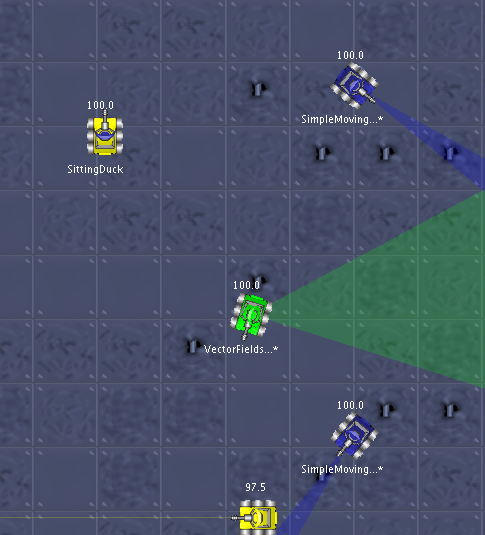
\includegraphics[width=0.8\textwidth]{images/FinalRun}
\caption{The final test for the Potential Field implementation features obstacles, both stationary and moving, and a moving goal.}
\label{Radar Lock Example}
\end{figure}

Each time the goal or an obstacle was scanned, onScannedRobot would grab the scanned objects name and insert an instance of the Enemy class into the HashMap. The Enemy class holds the calculated coordinate pair for the location of the scanned item as well as it's bearing at the time of the scan. The bearing was not used, but it was stored in case future modifications needed the additional information. This HashMap could then be iterated through in the navigation loop and the vectors could be calculated appropriately.

The potential fields implementation handled the course beautifully. When it would pass between obstacles, its speed would be dropped sufficiently to avoid any near collisions. It also handled the moving obstacle quite well, so long as the obstacle buffer was set sufficiently high. If it was set too low, often times the robot would not react in time to sudden directional changes from the obstacles and would be crashed into. 

Perhaps the only change I would make to this algorithm would be taking into consideration how much to scale the speed based on how many obstacles are affecting the tracking robot. Each drop in speed was calculated independently for each obstacle. So if the robot was within range of three obstacles, each one of those obstacles would cause its own drop in the tracking robot's speed. This meant that often times the robot's speed would drop significantly even if it wasn't especially close to any one obstacle. However, the performance was still quite smooth with the current implementation.

To finalize potential fields, it was decided that noise needed to be added to the model. Comparison really wouldn't be fair with the other methods if potential fields operated solely in an ideal environment. Noise was added in two ways. The first method added a random offset to the turning angle at a certain probability. As an example, twenty percent of the time the robot would slip $\pm 30^{\circ}$ when turning. The second method added small amounts of noise to the radar scans by adding or subtracting some $\epsilon$ from the calculated coordinate pair of the obstacle or goal.

The potential fields implementations handled the noise quite well. The slips, even when really large, did not impact the results nearly as much as expected. Mostly the navigation path got a bit jittery, but the results were never catastrophic. Similarly, the robot didn't have too difficult of a time handling the radar noise. The noise was fairly small in comparison to the range of the obstacles, so there were not any collisions as a result of this. The only time the radar scan noise caused any truly noticeable affects was when the noise was turned up extremely high. So long as the noise was reasonable--$\pm$ a few percent of the total distance to the object--then the effect was not significant enough to cause problems.

% Conclusion
\subsection{Conclusion}
Overall, the potential fields implementation handled the majority of the situations it was put into quite well. Initially, the simple implementation worked as a proof of concept but not much else. It moved terribly slow, but it found the goal nonetheless. Moving over to a moving goal showed the weaknesses present in the simple motion model. It made it hard to constantly follow the moving goal. In fact, it was pretty much guaranteed that the tracking would fail unless the robot was started in the middle of the course and the goal robot travelled a specific path. Additionally, the speed of the tracking robot couldn't be scaled with regards to its distance from the goal without running the risk that it would lose track of the goal.

The advanced motion model helped to smooth out the performance and addressed the issues made evident in the simple model tests. The radar locking experiment shows what the robot was capable of when it had perfect knowledge, and it showed the smoothest results when just dealing with a goal and no obstacles. It also demonstrated the speed adjustment with regards to distance from the goal best since it had perfect information on the goal. 

The obstacle avoidance results were quite good after the discovery of the advanced motion model. At first, expectations were low when watching the test runs with the simple motion model. However, the performance took off with the advanced motion model. Tracking a goal while dealing with an object was no challenge for the test bots. Even a moving goal with moving and stationary obstacles worked quite well.

Even with all the successes, there were still problems present with the method. The implementations had difficulty with congested environments, especially when it would attempt obstacle avoidance too near to a wall. This was especially evident with high \emph{MaxSpeed} settings. Often times the robot would sweep wide around an obstacle that was near a wall and collide. Unfortunately, with Robocode it isn't possible to detect the wall with the radar. It would be possible to simply generate a repulsive vector based on the coordinates of the robot with regards to the width and height of the arena; But that seemed a bit like cheating. Abusing the perfect world coordinates to the extent of making up readings didn't seem in the spirit of the tests.

Additionally, the method struggled with closely placed obstacles since it couldn't detect the optimal path around them. This is where the planning of the other methods could become beneficial. The reactionary behaviour of the potential fields could be used to subsume the long term thought out behaviour present in the alternative methods. This could create quite a robust system.

\section{Markov Decision Processes}
\label{Markov Decision Processes}
Discussion and plots...

\section{Q-learning}
\label{Q-learning}

Reinforcement learning is generally more computationally expensive,
less fine-grained, and less deterministic than other methods we've
examined. Given that these are all obvious downsides in a
real-time dynamic context, why is reinforcement learning worth
considering? Primarily, it brings the potential for a great deal of
flexibility in handling unknown environments, sensor quality, and
motion models. While, if other methods are possible they should likely
be the first choices, it does provide a valuable option in certain
cases.

\subsection{Setup}

The basic Robocode setup for Q-learning extends
the setup for MDPs. The basic structures of discretizing the state
space, discretizing robot movements, and handling the threading needed
for long-running processes were similar between the two methods.

Given the structure of the algorithm, the large transition tables of
the MDP approach were not required. The noise could be added on each movement
step during training and actual runs. As such, all we required was a
basic randomization method to send the bot on an incorrect path a
certain percentage of the time. This was kept the same as in the MDP
tests with an 80\% probability of following the selected route with a
10\% chance of slip with motion along either of the two adjacent
movement directions.

Basic rewards were structured similarly to the MDP trials. An action
which led into the goal state returned a reward of 100, an action
which caused motion into a
wall (or, later, an obstacle) gave a -100 reward, and all other
actions returned a reward of -1.

For policy visualization, we wrote a method in Matlab to take the output
policy and convert it into a quiver graph which proved useful for
visualization of all discrete policies.

\subsection{Experiments}

\subsubsection{Offline trials}
The first step was to confirm the functioning of the basic
Q-learning method. To do this, we ran initial tests with a fixed
starting point for the bot and a fixed, stationary
goal. The learning was run offline, a policy generated and
incorporated into a simple bot whose only processing was to determine
its current state and run the appropriate policy.

Initially these tests were run in a noiseless environment to
confirm basic operations of the various components. Adding in noise
produced distinctly rougher bot motion, but did not impact the overall
effectiveness of the method.

Both Boltzmann explorations and $\epsilon$-greedy were experimented
with at this phase.  We began by exploring the quality of the bots
given a similar numbers of trials. Here Boltzmann was clearly
superior, producing policies which more consistently and directly led
to the goal.

But the constraint was on computational time, not episodes so we
further ran a series of rough tests comparing along this axis. $\epsilon$-greedy method ran in approximately half the
time for a given number of trials (a ratio which seemed to scale with
the number of trials). So, at this point we compared $\epsilon$-greedy
with twice the number of trials against Boltzmann. Even in this case,
the overall policy produced by Boltzmann was better with fewer failure
incidents and better tracking performance.

While both were left in as options on all future
bots, Boltzmann was the default from this point on. The advantages in
overall performance and quality per unit of computational effort were
clear.

\subsubsection{Taking it online}

Things became a bit more complex as we shifted to
learning in the context of the environment itself. This required
several basic elements. First, the bot required the ability to scan
the environment for the location of the goal state. Second, the bot
required the ability to call out to the Q-learning method from inside
the Robocode environment. Finally, there needed to be a default policy
for the initial period when the bot had not yet learned a policy given
the environment. 

The most difficult part of this was dealing with a long-running
learning process in the context of the Robocode environment. As we
discussed in the MDP section, this was accomplished by spawning a
separate thread to run the learning process while a default random
policy was executed as the robot continued to scan the field.

For initial testing, we started the bot and goal in fixed points so
that we could control for the starting conditions. However, we were
quickly able to transition to randomly placing the two elements. The overall
performance on these tests was good. The bot could randomly move while
calculating its policy and then shift over to the resulting policy
once complete.

\subsubsection{Performance and dynamic environments}

At this point we shifted over to allowing for motion in the goal
state. Several issues became apparent at this point. The first was that, as we'd expected, the
speed of Q-learning was an issue in a dynamic environment. The numbers
of episodes we'd run in the offline tests or even in the
static tests were no
longer feasible. 

The first thing we tried was lowering the number of episodes. 
However, shifting this down to smaller numbers of episodes produced policies of a noticeably lower quality. In
particular, the bot had a tendency to get caught in state loops where
an incompletely learned policy would have two states which pointed to
one another. The other primary failure mode were states which directed
the bot directly into a wall.

Effectively, the number of episodes traded off fairly directly with
the quality of the policy. However, we were not able to implement a
precise way of tuning this relationship. We settled on 100,000 episode as a manageable
compromise. While not producing perfect episodes, it ran in under two
seconds (often closer to one) which was essential to
keeping tracking reasonably accurate. This would clearly be an area
for more detailed future exploration.

However, even that shortened learning time imposed a cost on the process. Notably, in
that period of time the bot (and, in later experiments, the goal)
could have shifted location rather dramatically. Several pieces were
needed to account for this.

First, we added a basic predictive aspect to the location of the goal
state. This meant accounting for its current velocity and bearing and
predicting where it would be after the policy was completed. However,
there were a number of issues with this method. The prediction itself
needed to account for the structure of the environment (walls, in
particular). Additionally, changes in direction by the goal could make
this approach directly maladaptive. While we kept experimenting with
this, past a certain point adding too much intelligence to the
prediction seemed to defeat the aim of the learning agent. Still, in
limited contexts this was a useful tool.

Second, we added a more robust method for recalculating policies. The
first method that was tried was recalculating each time the goal
was viewed. Simple locking was put in place so a new update thread was
only spawned if an update wasn't currently in progress. The downside
to this method was that it was precisely at points when the goal
hadn't been seen lately that an update was most necessary.

So, we extended this keep track of the last view of the goal and, if
that passed a certain count of turns to pause, scan the field for the
goal, and then learn a new policy. However, what proved best was to
simply always be recalculating the policy. Effectively, each time a
policy was produced, the goal would be scanned for and a new learning
process begun with the current location of bot and goal.

This led to the next major performance adjustment. In earlier trials,
we had attempted to learn a whole-field policy since, with a single
learning cycle to work with, we had to have as universal a policy as
possible. To accomplish this, starting positions of the bot were
randomized from episode to episode in order to maximize coverage of
the state space.

At this point, we shifted to focus the start position
on the current location of the bot in relation to the goal. The upside
of this was to produce policies that were generally more effective
given a limited number of learning episodes. The downside was that
failure modes were far more severe when entered. As can be seen in the
following policy areas away from the primary route from bot to goal
were nearly unlearned.

\vspace{.3in}

\begin{figure}[htbp]
  \centering
  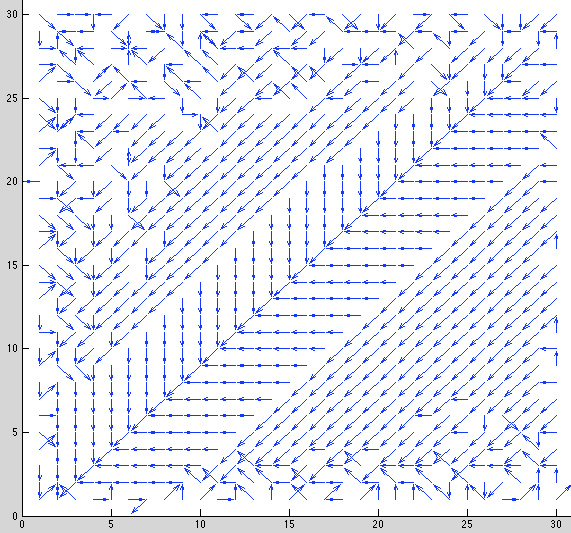
\includegraphics[width=\linewidth]{images/BasicPolicy.png} 
  \caption{Basic Q-learning generated policy.}
  \label{fig:basicQ}
\end{figure}
\clearpage

However, frequent updates proved an effective antidote to these
issues. In most cases, even when the robot was caught in a loop of
states, the next update would free it to continue tracking the goal.

\subsubsection{Obstacles}

The final major addition we made was to add obstacles to the
environment. In the first iteration of this, these were fixed and
pre-specified environmental features. At the next phase we moved to
allowing dynamic obstacles in the environment which the bot had to
scan and incorporate into its model.

The changes required to support this weren't huge. The bot had to be
capable of distinguishing obstacles from the goal and treating the two
differently. On the learning side, this required an adjustment to
reward model to account for obstacles in the learning
process. We treated obstacles as equivalent to walls with a -100
reward for colliding with an obstacle. An example of a policy which
accounts for obstacles (in this case, a wall in the lower left quadrant) can be
seen below.

\vspace{.3in}

\begin{figure}[htbp]
  \centering
  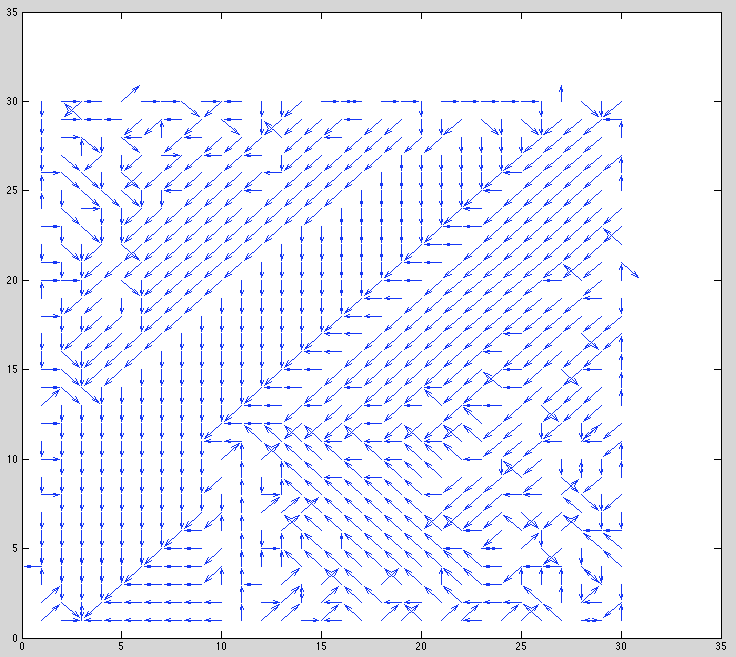
\includegraphics[width=\linewidth]{images/Wall2.png} 
  \caption{Q-learning generated policy with obstacles.}
  \label{fig:basicQ}
\end{figure}
\clearpage

There were several issues with this. Obstacles could shield one
another, preventing the back one from being scanned. This was
generally not an issue as, by the time the second obstacle was
reached, a new scan had generally taken place. More issues were caused
by the fact that the goal could also be shielded by an
obstacle. For this, the best we were able to do was constantly update
the goal location so that, even if it was hidden by an obstacle prior
to a new learning process, we would still have a reasonable estimate
of its position.

However, given all of the previous issues, moving obstacles proved
slightly too much for these methods. Beyond a certain amount of
complexity on the field, the updates were simply too slow to produce a
viable policy.

\subsubsection{Heuristic reward functions}

Two other experiments were tried that produced more ambiguous
results. First, we attempted to replace the reward function with a
heuristic based on euclidean distance to the goal. For smaller numbers
of episodes, this produced much better policies. The reason is that,
given the structure we'd set up, this method basically became a
search method. Effectively, at each step, it
would choose the step closest to the goal. For a single episode,
this would look like a depth-first search. In the simplified
environments we were working with, there would be little or no
backtracking required. Over a number of episodes, this would start to
look more like a best-first search, specifically A* given the use of a
valid heuristic function.

Surprisingly, the results were not better for this method with a larger
numbers of iterations. What we observed were policies that actually
gave less complete coverage of the state space. This can be seen in
the following policy which can be compared to Figure~\ref{fig:basicQ} (same
start and goal locations).

\vspace{.3in}

\begin{figure}[htbp]
  \centering
  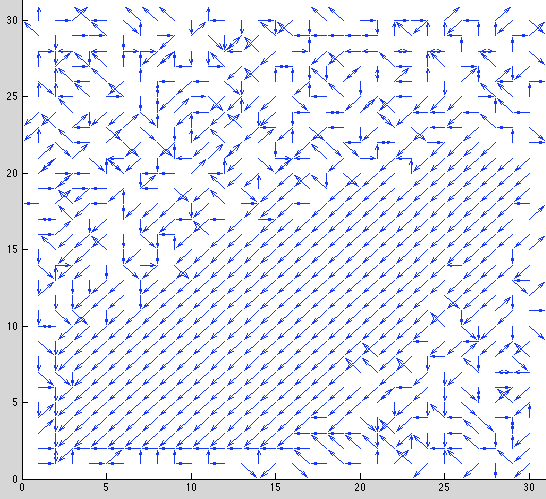
\includegraphics[width=\linewidth]{images/HeuristicPolicy.png} 
  \caption{Q-learning generated policy with a heuristic reward policy.}
  \label{fig:heurQ}
\end{figure}
\clearpage

This may well have been a result of exploration
not being properly tuned to the improvement in the reward
function. The heuristic reward, in pulling each step towards a greedy
depth-first approach, would require a more powerful push to exploration
to overcome the additional pull of the new reward function. The lack
of this may have led to a failure to explore
the state space as widely. Of course, if this type
of reward and environment information were available to an actual bot,
simply
running a true A* would be far more
efficient and could be updated real-time for such a highly discretized
space.

Finally, we explored variable grid sizes for the evaluation with the
aim being to run with a coarser grained grid the farther away from the
goal we were (once again, assuming that such information was
accessible to the model which, in reality, would likely open up other
methods). Unfortunately, we weren't able to get this piece working
correctly by the deadline.

\subsection{Evaluation}

The largest issue with our implementation of Q-learning is that it
relies on information which, if present, could better drive a more
efficient and/or complete method. By pulling information about the
field into what amounts to a local simulation in which the learning
takes place, we undercut much of the real-world justification for the
use of a learning method. However, our aim was to consider these
methods primarily for future use (Robocode, while charming, is not the
end goal for any of us). In that context, our results suggest certain
more interesting elements.

First, we must note that, as expected, Q-learning is not an ideal method for the type of
conditions we set up for these experiments. It's update time is too
slow, policies are far less efficient, and it can easily get caught in
local state loops. Moreover, the method proved somewhat brittle, in
many cases failing completely. This seemed to be an interaction with
the Robocode environment. For example, when an incorrect policy would
have the bot attempt to repeatedly ram a wall, Robocode would at times
disable the bot.

However, while certainly not the best choice, the more surprising
result is that we were able to get Q-learning running well-enough to
successfully operate in a dynamic real-time environment at all. The
fact that policy updates could be recomputed on the fly fast enough to
maintain tracking on a moving goal was interesting and somewhat
surprising. We'd expected that this method would have to be used
largely offline with policies generated and fed in. Being able to get
it to the point of updating while in a dynamic environment was a surprise.

In particular, what this suggests several ways that Q-learning might serve as a
component of an overall navigation system. One possibility would be as
part of an overall voting system. Especially given a noisy
environment, a learning method could provide a needed bias among
competing focused heuristics.

A better approach would likely be a hybrid system. For example, say
there were a number of different standard goal movement patterns, but
these were obscured by uncertainty in motion, shifting environmental
conditions, etc. A learning method combined with more straightforward
predictive modeling of the other bots could potentially help to
account for that noise. Action choices would still be managed through
more efficient methods, but the choice among those methods handled by
a learned evaluation over a given set of state parameters.

One area where more work is definitely needed is on reward function
optimization. Clearly there is a great deal of tweaking and rebalancing
possible, but we were not able to fully explore the implications of
this.

However, our experiment on shifting from fixed rewards to
heuristic rewards provided some interesting hints as to future possibilities. First, the hidden cost of
adding information into the reward in terms of overwhelming the
pressure to explore was not something we expected. 

It
emphasized the need for improved reward information to be combined with a greater emphasis
on exploration. Uncertainty in the system (from both sensors and
motions) has to be reflected in the learning process. If that process
effectively learns as though the environment were purely
deterministic, the resulting policy will be unlikely to respond
correctly when acted on in that environment.

Additionally, it
suggested some interesting possibilities in terms of injecting
additional information into learning methods as a way to take
advantage of additional information if present. This might be
especially useful in a situation where such information were only
sporadically present. For example, a noisy sensor which sporadically
gave a distance measure could be incorporated, but with the awareness
that additional weight might need to be given to exploration to
balance this out in a learning context.

The central theme in our exploration of Q-learning in a dynamic
context was one of tradeoffs. While this and related reinforcement
learning methods are extremely powerful and flexible (most of that power
left untapped in this case), the tradeoffs involved in their application
seem to strongly call for use in combination with other
methods. Applied properly, those strengths can be exploited while the weaknesses
are shored up by other methods.

\section{Conclusion}
\label{Conclusion}
To sum up...

\subsection{Future work}

\section{Acknowledgments}
Our team would thank Franz Kafka, Alan Turing, and the Ghost of
Christmas Past for their unwavering support during this project. We
would also like to pour a drink for our homies in the ground.


% \bibliographystyle{aiaa}

% \bibliography{References_Database_Daoru}

\end{document}
